y\section{Problem}

The Medical test Records project approaches two main issues that hospital information systems face. \\

The first, is how the sensitive information must be stored,  and who should have access to it in order for the hospital staff (the doctors, nurses, assistants, etc...) provide the patients with the adequate treatment without making the patient's private information available to everyone.
A patient profile has associated with it a group of information with different levels of sensitivity, such as age, name, blood type, diseases, family records and others.
A patient's name is not extremely sensitive so most employees can access it. However, for instance,the patient's family records do not need to be accessed nor should be accessible to most of the hospital staff, for example to volunteers. \\

Given this scenario, the information systems  must be able to provide and enforce the correct policies so that different parts of a patient's profile are only available to whom actually requires them to fulfill one's obligations to the patient, relating to the role performed and in the correct context. \\

The second problem comes from medical tests being analyzed in different facilities, like partner labs, that are not part of the hospital infrastructure, but require that both are interconnected in a way that enables all sides to identify each other and communicate in a safe and secure way. \\

\subsection{Requisites}

Given the previous problems, the implementation of this project requires the following security guarantees:
\begin{itemize}
	\item A fine grained access control and secure authentication mechanism.
	\item Authenticity of all communications with the information systems.
	\item Confidentiality of all communications with the information systems.
	\item Non-repudiation and integrity of the test results data.
\end{itemize}

\subsection{Trust assumptions}


There are three main entities in this project which are the hospital information system, the labs and the staff that uses said systems. \\

The hospital information system which will store all of the patient data and tests results received from the labs. The partners labs that will communicate with the hospital and vice-versa throught their respective API's. And finally the users of those systems, the staff. In case of the staff there is a full trust assumption that they won't have their credentials stolen/shared/etc., and as such we will not provide any mechanism to rapidly revoke those credentials. \\

All communications will use HTTPS requests, and will be considered secure and resistant against attacks like replay, tampering and eavesdropping. \\

There is also a full trust assumption, that all the code responsible for the access control, libraries used and frameworks are error free and won't give any type of access to an attacker. \\


\section{Proposed solution}

The implementation will be separated in two main components, an hospital REST API and a laboratory REST API, which will act as client or server, depending on the action being done. When further mentioned API in this text both the hospital's API and lab's API's are being referred to, as they will be pretty similar in terms of security and access control. The only difference between those two entities (hospital and labs) API's, are the possible actions and data stored. \\

All communications between those systems will run with TLS to provide confidentiality, integrity and freshness. TLS will be provided by the Spring framework, which will be used to develop the API. \\

	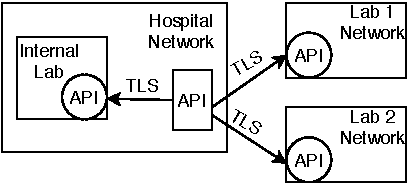
\includegraphics[width=.4\textwidth]{figs/infrastructure.pdf}
	
TLS will require the definition of a certificate for each entity, we will consider that the certificates are installed manually by an administrator on each respective machine.
We will have a made-up CA, which we will use to issue and sign the hospital's certificate and each lab's certificate (including labs inside the hospital). Those certificates alongside with the secure communication channel, will be used to digitally sign the sent tests data to guarantee its authenticity at any time.
In order to validate the certificate received by the server during the TLS Handshake, each machine will have the root CA certificate already installed, manually, by an administrator.\\ 

All requests received by the API need to posess a proof of identity to be further processed (accept or refuse action), in this case will be a token provided by the respective entity API, after authentication using the correct set of credentials (username:password). The token is transported in the "Authorization" header of the HTTP request. If the token is not present the request will be refused with status code 401 UNAUTHENTICATED. \\

If the request contains all necessary information (token), it will be forwarded to the access control mechanism. \\

The access control mechanism is composed by 4 major components:
\begin{itemize}
	\item PEP - Policy Enforcement Point
	\item PDP - Policy Decision Point
	\item PAP - Policy Administration Point
	\item Policy Store
\end{itemize}

The PEP will send a XACML request to the PDP, the PDP will then based on the policies defined by the system return a XACML response which will dictate the action (ACCEPT or REFUSE) that PEP will enforce. If the result is ACCEPT, the request will continue and read or write the requested resource, otherwise the request will be dropped and replied with a 403 UNAUTHORIZED.

	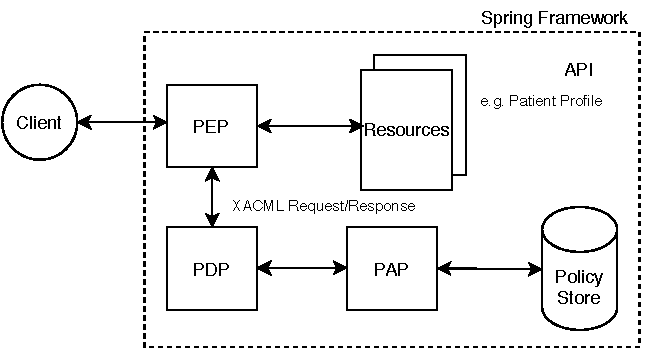
\includegraphics[width=.6\textwidth]{figs/access_control.pdf}
	

\section{Plan}

\subsection{Basic}
The basic version of the project must have the following components in place:
\begin{itemize}
	\item API.
	\item TLS for secure communication channels.
	\item Access Control.
\end{itemize}

It is expected that this version will take around 2 weeks to complete (worst case scenario). 


\subsection{Intermediate}
The intermediate version will expand what was built in the first 2 weeks adding the following:
\begin{itemize}
	\item The necessary mechanism to check tests data authenticity at any time. (Digital Signature)
	\item Sensitive information like passwords stored in a safe way (hashed).
	\item Correct any bugs or misconfigurations left in the access control and TLS.
\end{itemize}

This phase should take around 1 week.


\subsection{Advanced}

By this point the necessary mechanisms are all implemented, possible bugs should be corrected now, if there are none, the project can take a step further and do the following to increment the security or optimize the system:

\begin{itemize}
	\item Encryption of all the confidential information in the database, to avoid leaks in case of a breach.
	\item Policies and authentication information cache. (Will avoid constant reads to the database everytime there is a request).
	\item Defining rule combining algorithms in the access control for  more complex decisions.
	\item Firewall implementation.
\end{itemize}


\subsection{Effort Commitment}

\begin{tabularx}{0.8\textwidth} { 
  | >{\centering\arraybackslash}X 
  | >{\centering\arraybackslash}X 
  | >{\centering\arraybackslash}X 
  | >{\centering\arraybackslash}X | }
 \hline
  & Alexandru & Ana Marta & Rafaela \\
 \hline
 Week 1  & API & Deployment Scripts & Database \\
  \hline
  Week 2  & Access Control  & TLS & Tests data authenticity mechanism \\
   \hline
   Week 3  & Access Control  & TLS  & Tests data authenticity mechanism \\
    \hline
    Week 4  & Firewall  & Rule Combining Algorithms  & Database encryption \\
\hline
\end{tabularx}

\section{References}

The project client and API infrastructure will be developed using the Java programming language. \\

The API will use the \href{https://docs.spring.io/spring-framework/docs/3.2.x/spring-framework-reference/html/mvc.html}{Spring Web MVC} Framework to attend and process the client requests, enable the TLS communications and manage the KeyStores (Hospital certificate) and TrustStores (partner labs certificates). \\

The deployment scripts will use \href{https://www.vagrantup.com/}{Vagrant} to manage and deploy the VM's with the correct network configurations and all the necessary software to run the applications. \\

The database management system will be provided by \href{https://www.mysql.com/}{MySQL}. \\

The access manager architecture and policy defining language to be implemented is specified by OASIS eXtensible Access Control Markup Language \href{https://www.oasis-open.org/committees/tc_home.php?wg_abbrev=xacml#other}{(XACML)}. For the policy definition it will be used the JSON XACML Profile. \\

Finally, the certificates will be self-signed and created using \href{https://www.openssl.org/}{OpenSSL}. \\
